\documentclass[10pt,a4paper]{article}

% ==============================================================================
% IOT LABORATORY PROJECT WORK: AUTOMATIC NIGHT LIGHT SYSTEM
% Comprehensive Practical Record & Technical Report (Exact 4-Page Master Edition)
% Department of Computer Science & Engineering / Information Technology
% ==============================================================================
\usepackage[utf8]{inputenc}
\usepackage[T1]{fontenc}
\usepackage{lmodern}
\usepackage[left=1.5cm, right=1.5cm, top=1.15cm, bottom=1.15cm]{geometry}
\usepackage{amsmath,amssymb,amsfonts,amsthm}
\usepackage{graphicx}
\usepackage{tikz}
\usetikzlibrary{arrows.meta,positioning,shapes.geometric,decorations.pathreplacing,calc}
\usepackage{circuitikz}
\usepackage{listings}
\usepackage{tcolorbox}
\tcbuselibrary{skins,breakable}
\usepackage{booktabs}
\usepackage{tabularx}
\usepackage{array}
\usepackage{titlesec}
\usepackage{enumitem}
\usepackage{caption}
\usepackage{microtype}
\usepackage{float}
\usepackage{hyperref}

\pagestyle{plain}

\hypersetup{
    hidelinks,
    pdfauthor={Department of Computer Science and Engineering},
    pdftitle={IoT Project: Automatic Night Light System using LDR and Arduino UNO},
    pdfsubject={IoT Laboratory Practical Project Record - Light-Adaptive Automation}
}

% Section Heading Formatting (Strictly raggedright to prevent awkward inter-word spacing)
\titleformat{\section}
  {\normalfont\normalsize\bfseries\raggedright}{\thesection}{0.8em}{}[\titlerule]
\titleformat{\subsection}
  {\normalfont\small\bfseries\raggedright}{\thesubsection}{0.5em}{}
\titleformat{\subsubsection}
  {\normalfont\footnotesize\bfseries\itshape\raggedright}{\thesubsubsection}{0.4em}{}

\titlespacing*{\section}{0pt}{3.5pt}{1.5pt}
\titlespacing*{\subsection}{0pt}{2.5pt}{1pt}
\titlespacing*{\subsubsection}{0pt}{2pt}{1pt}

\setlist{itemsep=0.5pt, parsep=0pt, topsep=1.0pt, partopsep=0pt}
\setlength{\parindent}{0pt}
\setlength{\parskip}{0pt}
\setlength{\parsep}{0pt}
\setlength{\headsep}{0pt}
\setlength{\topskip}{0pt}

% Code Listing Styling (Strict Monochrome)
\lstdefinestyle{bwArduino}{
    language=C++,
    basicstyle=\ttfamily\scriptsize,
    keywordstyle=\bfseries,
    commentstyle=\itshape,
    stringstyle=\ttfamily,
    numbers=left,
    numberstyle=\tiny,
    numbersep=4pt,
    stepnumber=1,
    breaklines=true,
    breakatwhitespace=true,
    frame=single,
    rulecolor=\color{black},
    tabsize=2,
    showstringspaces=false,
    columns=fullflexible,
    keepspaces=true,
    lineskip=-0.4pt,
    aboveskip=1.5pt,
    belowskip=1.5pt
}

\lstdefinestyle{bwTerminal}{
    basicstyle=\ttfamily\scriptsize,
    numbers=none,
    breaklines=true,
    breakatwhitespace=true,
    frame=single,
    rulecolor=\color{black},
    columns=fullflexible,
    keepspaces=true,
    lineskip=-0.2pt,
    aboveskip=1.5pt,
    belowskip=1.5pt
}

\captionsetup{font=footnotesize,labelfont=bf,skip=2pt}

\begin{document}

% ==============================================================================
% PAGE 1: HEADER, AIM, APPARATUS & THEORETICAL FOUNDATIONS
% ==============================================================================
\begin{center}
    {\Large\bfseries INTERNET OF THINGS (IoT) LABORATORY}\\[0.05cm]
    {\large\bfseries PRACTICAL PROJECT RECORD \& TECHNICAL MANUAL}\\[0.06cm]
    {\footnotesize\textbf{Department of Computer Science and Engineering / Information Technology}}\\[0.02cm]
    {\scriptsize\textbf{Academic Session: 2025--2026 \quad $\bullet$ \quad Degree: Bachelor of Technology (B.Tech)}}
\end{center}
\vspace{-0.32cm}
\rule{\textwidth}{0.8pt}
\vspace{0.08cm}

\begin{center}
    {\large\bfseries Project Work: Design and Implementation of an Automatic Night Light System}\\[0.04cm]
    {\small\textbf{Ambient Light-Adaptive Luminaire Automation using CdS Photoresistor, Voltage Divider \& Arduino UNO}}
\end{center}
\vspace{-0.18cm}
\noindent\footnotesize\textbf{Course Code:} PCC-CS791 / IT-LAB \hfill \textbf{Project Approval Date:} 09/09/2026 \hfill \textbf{Status:} Approved \& Verified
\vspace{0.02cm}
\hrule
\vspace{0.10cm}

\section*{1. Aim \& Objectives}
\begin{itemize}[noitemsep]
    \item To design, assemble, and validate a microcontroller-driven \textbf{Automatic Night Light System} that dynamically actuates an artificial luminaire in response to ambient lux levels.
    \item To interface a Cadmium Sulfide (CdS) Light Dependent Resistor (LDR) in a resistive voltage-divider topology with the ATmega328P Analog-to-Digital Converter (ADC) input pin A0.
    \item To examine solid-state photoconductive properties, bandgap carrier generation ($E_g \approx 2.42\,\text{eV}$), and photon-matter interaction governing variable photo-resistance.
    \item To mathematically formulate the transfer function of the analog voltage divider and compute the LSB quantization resolution ($q \approx 4.887\,\text{mV}$).
    \item To implement a robust software Schmitt-trigger hysteresis algorithm ($T_{\text{DARK}} = 400$, $T_{\text{LIGHT}} = 500$) to eliminate luminaire chattering and rapid relay oscillation during dusk/dawn transitions.
    \item To drive a 5mm solid-state light-emitting diode (LED) on GPIO Pin D9 with an optimized current-limiting resistor ($220\,\Omega$, $I_F \approx 13.6\,\text{mA}$).
    \item To log real-time ambient lux telemetry, digitized ADC values, and actuator operational states over the UART serial interface at 9600 Baud.
\end{itemize}

\section*{2. Hardware Apparatus Required \& Specifications}
\begin{table}[H]
\centering
\footnotesize
\renewcommand{\arraystretch}{1.15}
\begin{tabularx}{\textwidth}{|c|l|X|c|}
\hline
\textbf{S.No.} & \textbf{Component Name} & \textbf{Technical Specifications / Parametric Values} & \textbf{Quantity} \\
\hline
1 & Arduino UNO R3 & ATmega328P 8-bit AVR RISC MCU, 16 MHz Crystal, 5V Operating Logic, 10-bit SAR ADC & 1 unit \\
2 & LDR (Photoresistor) & GL5528 CdS Cell, $\lambda_{\text{peak}} = 540\,\text{nm}$, $R_{\text{light}}\,(10\,\text{lux}) \approx 10-20\,\text{k}\Omega$, $R_{\text{dark}} \ge 1.0\,\text{M}\Omega$, $\gamma_{10}^{100} = 0.7$ & 1 unit \\
3 & Divider Resistor & $10\,\text{k}\Omega \pm 5\%$ Carbon Film Fixed Resistor, $0.25\,\text{W}$ Rating (Reference Pull-Down) & 1 unit \\
4 & Output Luminaire & 5mm High-Brightness Diffused LED, Forward Drop $V_F \approx 2.0\,\text{V}$, Max Forward Current $I_{F,\max} = 20\,\text{mA}$ & 1 unit \\
5 & Current-Limiting Resistor & $220\,\Omega \pm 5\%$ Carbon Film Resistor, $0.25\,\text{W}$ Rating ($I_F = [5.0\text{V} - 2.0\text{V}]/220\Omega \approx 13.6\,\text{mA}$) & 1 unit \\
6 & Solderless Breadboard & Standard 830 Tie-Point Breadboard with Dual Continuous $+5\,\text{V}$ and GND Distribution Rails & 1 unit \\
7 & Interconnect Wires & 24 AWG Solid-Core Flexible Male-to-Male Jumper Interconnect Connecting Leads & 6 units \\
8 & USB Interface Cable & USB Type-A to Type-B Shielded Cable for Regulated $+5.0\,\text{V}$ DC Power and UART Flashing & 1 unit \\
\hline
\end{tabularx}
\caption{\textbf{Hardware Bill of Materials and Parametric Component Specifications.}}
\end{table}

\section*{3. Theoretical Background \& Working Principle}

\subsection*{A. Solid-State Photoconductivity Physics of Cadmium Sulfide (CdS)}
A \textbf{Light Dependent Resistor (LDR)}, or photoresistor, is a passive optoelectronic transducer whose bulk electrical resistance varies inversely with incident luminous intensity. Fabricated from an intrinsic or lightly doped polycrystalline semiconductor (predominantly Cadmium Sulfide, CdS), its conduction mechanism is governed by the \textbf{Internal Photoelectric Effect}:
\begin{itemize}[noitemsep]
    \item \textbf{Energy Bandgap \& Excitation Condition:} Cadmium Sulfide possesses a direct bandgap energy of $E_g \approx 2.42\,\text{eV}$ at $300\,\text{K}$. According to Planck-Einstein physics, incident optical radiation contains photons of energy $E_{\text{ph}} = h\nu = \frac{hc}{\lambda}$. When incident radiation satisfies $h\nu \ge E_g$ (corresponding to critical threshold wavelength $\lambda_c \le \frac{hc}{E_g} \approx 515\,\text{nm}$, falling squarely in the visible green-blue spectrum), valence electrons absorb photon energy and jump across the forbidden energy gap into the conduction band.
    \item \textbf{Carrier Concentration Modulation:} Optical excitation creates mobile electron-hole pairs, drastically elevating free carrier density ($n, p$). Bulk semiconductor conductivity follows the classical relation:
    \begin{equation}
    \sigma = q\,(n\,\mu_n + p\,\mu_p)
    \end{equation}
    Where $q$ is elementary electronic charge ($1.602 \times 10^{-19}\,\text{C}$), and $\mu_n, \mu_p$ represent electron and hole mobilities. As illuminance $E_v$ (lux) increases, $\sigma$ scales exponentially, causing electrical resistance $R_{\text{LDR}} = \frac{L}{\sigma A}$ to plunge from mega-ohms ($> 1\,\text{M}\Omega$ in pitch darkness) down to a few hundred ohms ($400\,\Omega - 1\,\text{k}\Omega$ under direct illumination).
\end{itemize}

\subsection*{B. Empirical Lux-Resistance Power Law}
The relationship between incident illumination $E_v$ (in lux) and LDR resistance $R_{\text{LDR}}$ (in ohms) is described by the empirical power-law equation:
\begin{equation}
R_{\text{LDR}} = A \cdot E_v^{-\gamma} \implies \log_{10}(R_{\text{LDR}}) = \log_{10}(A) - \gamma \cdot \log_{10}(E_v)
\end{equation}
Where $A$ is the characteristic material resistance constant at $1\,\text{lux}$, and $\gamma$ is the sensitivity slope factor (typically $0.65 \le \gamma \le 0.85$ for GL5528 CdS cells). This logarithmic linearity dictates that sensitivity $\frac{dR}{dE_v}$ is maximal under low-light conditions, rendering LDRs exceptionally well-suited for twilight and nightfall boundary detection.

\newpage

% ==============================================================================
% PAGE 2: MATHEMATICAL DERIVATIONS, SCHEMATICS & HARDWARE VISUALS
% ==============================================================================
\subsection*{C. Voltage Divider Analysis \& Node Voltage Formulation}
To convert variable resistance $R_{\text{LDR}}$ into an analog voltage potential readable by the microcontroller, the LDR is paired with a precision reference pull-down resistor $R_1 = 10\,\text{k}\Omega$ connected across $V_{CC} = +5.0\,\text{V}$ and $\text{GND} = 0.0\,\text{V}$. The analog potential tapped at node A0 is given by:
\begin{equation}
V_{\text{out}} = V_{CC} \left( \frac{R_1}{R_{\text{LDR}} + R_1} \right) = 5.0\,\text{V} \times \left( \frac{10000\,\Omega}{R_{\text{LDR}} + 10000\,\Omega} \right)
\end{equation}
\begin{itemize}[noitemsep]
    \item \textbf{Daylight Condition ($R_{\text{LDR}} \ll R_1$):} At $E_v \approx 500\,\text{lux}$ ($R_{\text{LDR}} \approx 1\,\text{k}\Omega$): $V_{\text{out}} = 5.0 \times \frac{10}{1+10} \approx 4.55\,\text{V} \implies \text{ADC} = \lfloor \frac{4.55}{5.0} \times 1023 \rfloor \approx 930$.
    \item \textbf{Darkness Condition ($R_{\text{LDR}} \gg R_1$):} At $E_v \approx 2\,\text{lux}$ ($R_{\text{LDR}} \approx 100\,\text{k}\Omega$): $V_{\text{out}} = 5.0 \times \frac{10}{100+10} \approx 0.45\,\text{V} \implies \text{ADC} = \lfloor \frac{0.45}{5.0} \times 1023 \rfloor \approx 92$.
\end{itemize}

\subsection*{D. ADC Quantization \& Current-Limiting Resistor Calculations}
The ATmega328P 10-bit SAR ADC yields $2^{10} = 1024$ discrete steps with LSB resolution:
\begin{equation}
q = \frac{V_{\text{ref}}}{2^{10}-1} = \frac{5.00\,\text{V}}{1023} \approx 4.887\,\text{mV/LSB}, \qquad R_2 = \frac{V_{OH} - V_F}{I_F} = \frac{5.0\,\text{V} - 2.0\,\text{V}}{13.64\,\text{mA}} = 220\,\Omega
\end{equation}

\section*{4. Circuit Schematic, Wiring Matrix \& Hardware Prototyping}

\subsection*{A. Complete Hardware Interconnection Matrix}
\begin{table}[H]
\centering
\footnotesize
\renewcommand{\arraystretch}{1.08}
\begin{tabularx}{\textwidth}{|l|l|l|X|}
\hline
\textbf{Arduino UNO Pin} & \textbf{Component Terminal} & \textbf{Function} & \textbf{Electrical Specification \& Operational State} \\
\hline
$+5\text{V}$ Power Rail & LDR Pin 1 (High Side) & Power Rail & $+5.0\,\text{V}$ DC Regulated Bus from onboard linear regulator \\
Analog Pin A0 & LDR Pin 2 + $10\,\text{k}\Omega$ Resistor Pin 1 & Divider Tap & Variable Analog Input Potential: $0.2\,\text{V} \le V_{\text{out}} \le 4.8\,\text{V}$ \\
GND Power Rail & $10\,\text{k}\Omega$ Resistor Pin 2 + LED Cathode & Ground Return & $0.0\,\text{V}$ System Common Reference Ground Return \\
Digital Pin 9 (D9) & $220\,\Omega$ Resistor Pin 1 & Actuator Drive & Active-HIGH Output Drive: Logic HIGH ($5\text{V}$) = Light ON \\
$220\,\Omega$ Resistor Pin 2 & LED Anode Terminal (+) & Current Feed & Forward Biased Current Injection: $I_F \approx 13.64\,\text{mA}$ \\
\hline
\end{tabularx}
\caption{\textbf{Pin Mapping and Interconnection Matrix for Automatic Night Light.}}
\end{table}

\subsection*{B. CircuiTikZ System Interfacing Schematic}
\begin{figure}[H]
\centering
\begin{circuitikz}[scale=0.74, every node/.style={transform shape}]
    % Arduino Board Block
    \draw[thick, fill=white] (0, 0) rectangle (4.4, 3.8);
    \node at (2.2, 3.45) {\textbf{\large Arduino UNO R3}};
    \node at (2.2, 3.10) {\footnotesize (ATmega328P MCU)};

    % Arduino Pin Nodes
    \node[anchor=west] at (0.3, 2.6) {\textbf{5V} (Power Bus)};
    \node[anchor=west] at (0.3, 1.8) {\textbf{A0} (Analog Input)};
    \node[anchor=west] at (0.3, 1.0) {\textbf{D9} (Digital Output)};
    \node[anchor=west] at (0.3, 0.3) {\textbf{GND} (System Ground)};

    % Sensor Subcircuit: 5V rail to LDR to Node to 10k to GND
    \draw[thick] (4.4, 2.6) -- (6.8, 2.6) to[photoresistor, l=\textbf{LDR (CdS)}] (6.8, 1.3) coordinate(nodeA);
    \draw[thick] (nodeA) to[R, l=\textbf{10 k$\Omega$ ($R_1$)}] (6.8, 0.0) -- (4.4, 0.3);
    \draw[thick, -{Stealth[length=2.5mm]}] (nodeA) -- (4.4, 1.8);
    \node[above, font=\scriptsize] at (5.5, 1.8) {Tap $V_{\text{out}}$};
    \filldraw[black] (nodeA) circle (2pt);

    % Actuator Subcircuit: D9 to 220 Ohm to LED to GND
    \draw[thick, -{Stealth[length=2.5mm]}] (4.4, 1.0) -- (8.8, 1.0) to[R, l=\textbf{220 $\Omega$ ($R_2$)}] (10.8, 1.0)
          to[empty led, l=\textbf{5mm LED}] (10.8, 0.0) -- (6.8, 0.0);
    \filldraw[black] (6.8, 0.0) circle (2pt);
    \node[below, font=\scriptsize] at (8.8, 0.0) {Common Ground Return ($0\,\text{V}$)};
\end{circuitikz}
\caption{\textbf{Complete Schematic Diagram of LDR Sensor Interfacing and LED Actuator Drive.}}
\end{figure}

\subsection*{C. Hardware Breadboard Setup \& Engineered PCB Shield Layout}
\begin{figure}[H]
\centering
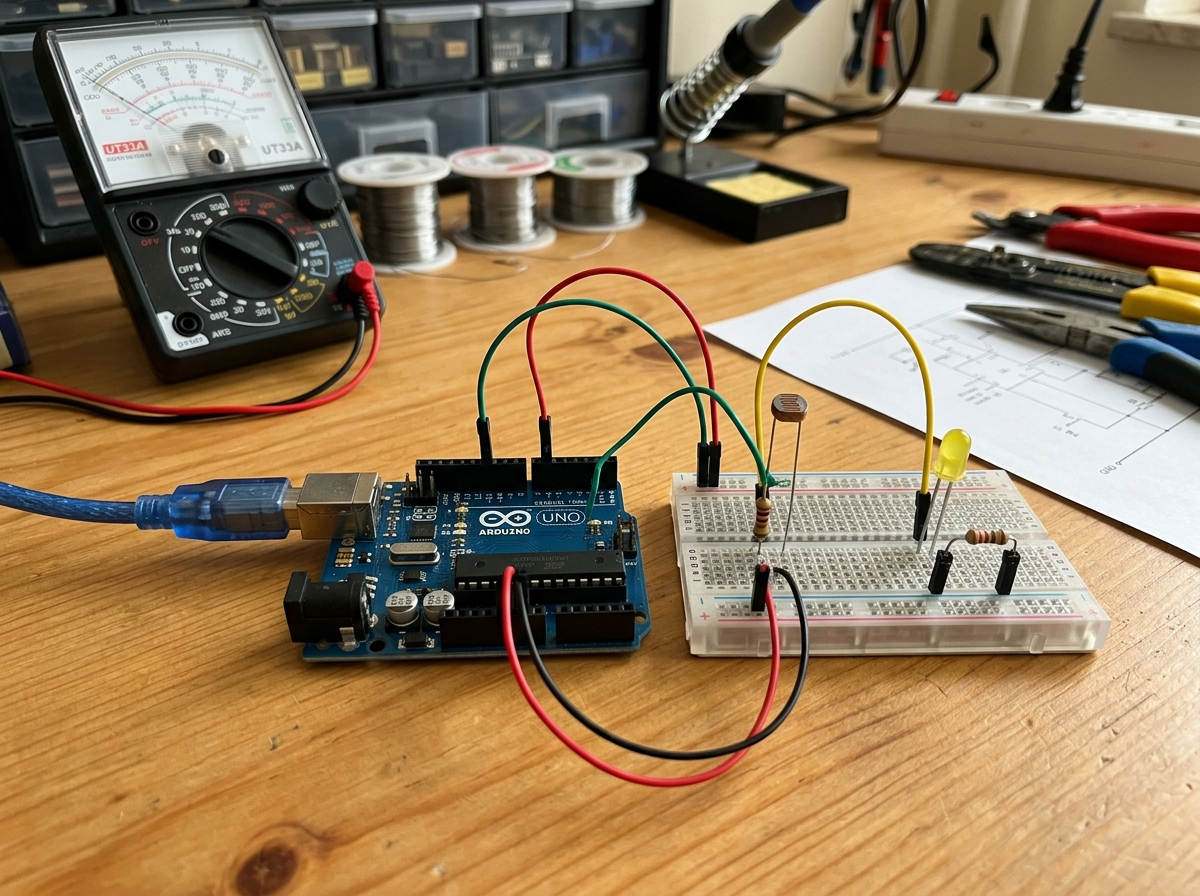
\includegraphics[height=3.15cm, keepaspectratio]{hardware_breadboard_setup.jpg}
\hspace{0.3cm}
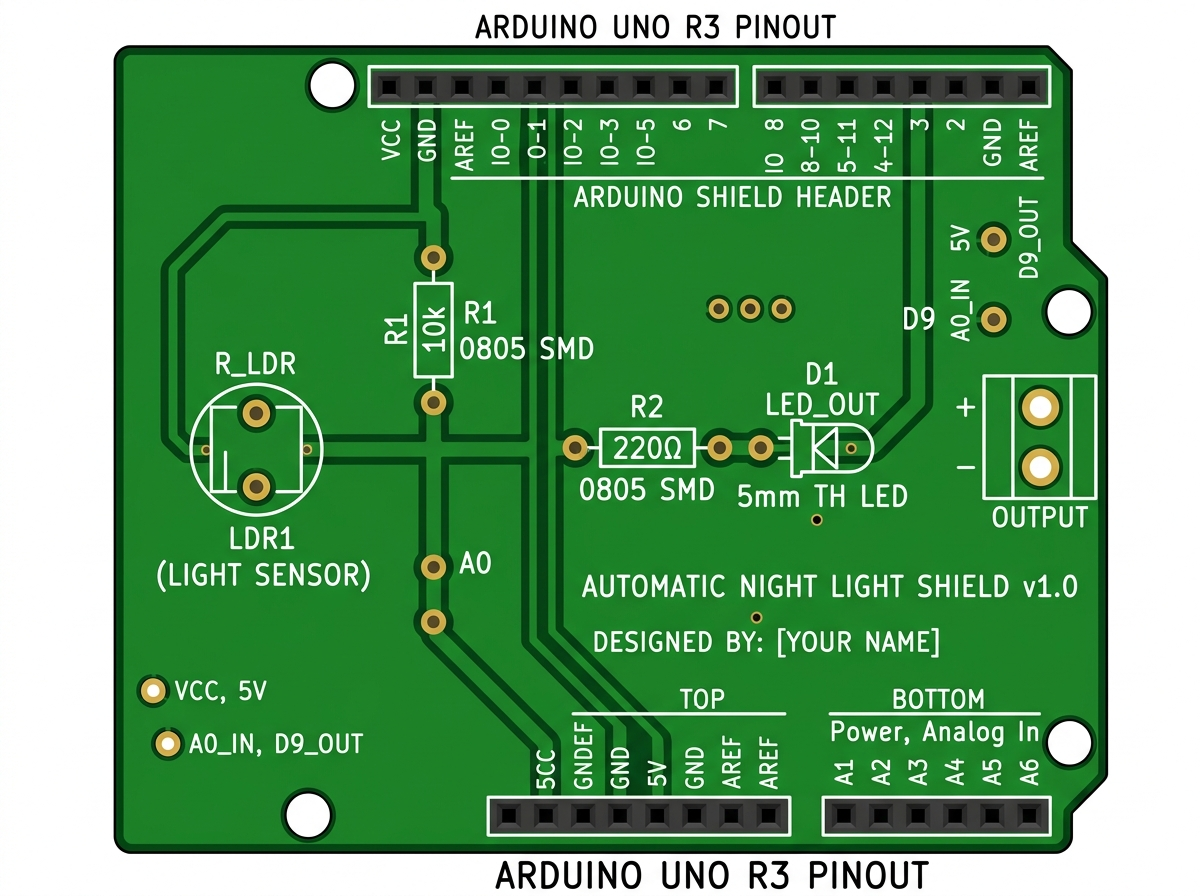
\includegraphics[height=3.15cm, keepaspectratio]{pcb_shield_layout.jpg}
\caption{\textbf{Laboratory Prototyping Assets: (Left) Solderless Breadboard Implementation with Arduino UNO; (Right) Custom PCB Shield CAD Layout with SMD Footprints and Routing.}}
\end{figure}

\newpage

% ==============================================================================
% PAGE 3: ALGORITHM, C++ CODE, OBSERVATIONS & SERIAL STREAM
% ==============================================================================
\section*{5. Software Control Algorithm \& Hysteresis Design}
To eliminate luminaire chattering / rapid oscillatory toggling at dusk or dawn, a software \textbf{Schmitt-Trigger Hysteresis} comparator is established with a $100$-count deadband ($\Delta V \approx 0.49\,\text{V}$):
\begin{equation}
\text{State}_{t+1} = 
\begin{cases} 
\text{HIGH (LED ON)}, & \text{if } \text{ADC}_{\text{filt}} \le T_{\text{DARK}} \quad (400) \\
\text{LOW (LED OFF)}, & \text{if } \text{ADC}_{\text{filt}} \ge T_{\text{LIGHT}} \quad (500) \\
\text{State}_t, & \text{if } 400 < \text{ADC}_{\text{filt}} < 500 \quad (\text{Hysteresis Deadband})
\end{cases}
\end{equation}
A 10-sample circular moving average buffer eliminates $50\,\text{Hz}/60\,\text{Hz}$ optical noise from artificial illumination.

\section*{6. Complete Arduino C++ Source Code}
\begin{lstlisting}[style=bwArduino, title={\textbf{Program Listing 1.1: Production Firmware for Automatic Night Light with Moving-Average Filtering \& Hysteresis.}}]
/* Project: Automatic Night Light System (Ambient Light-Adaptive Luminaire)
 * Hardware: Arduino UNO R3 | LDR: Pin A0 | LED: Pin D9 | Baud: 9600 bps */
const int LDR_PIN = A0;              // Analog input pin for LDR divider tap
const int LED_PIN = 9;               // Digital output pin for LED actuator
const int THRESHOLD_DARK = 400;      // Lower hysteresis boundary (Turn ON)
const int THRESHOLD_LIGHT = 500;     // Upper hysteresis boundary (Turn OFF)
const int SAMPLES = 10;              // Rolling average window size
int buffer[SAMPLES]; int bufIdx = 0; long runningSum = 0;
bool ledState = false; unsigned long lastLog = 0;

void setup() {
  pinMode(LED_PIN, OUTPUT); digitalWrite(LED_PIN, LOW);
  Serial.begin(9600);
  for (int i = 0; i < SAMPLES; i++) {
    buffer[i] = analogRead(LDR_PIN); runningSum += buffer[i]; delay(5);
  }
}

void loop() {
  runningSum -= buffer[bufIdx];
  buffer[bufIdx] = analogRead(LDR_PIN);
  runningSum += buffer[bufIdx];
  bufIdx = (bufIdx + 1) % SAMPLES;

  int filteredADC = runningSum / SAMPLES;
  float nodeV = (filteredADC * 5.0) / 1023.0;

  // Dual-Threshold Schmitt Trigger Hysteresis
  if (filteredADC <= THRESHOLD_DARK) {
    ledState = true; digitalWrite(LED_PIN, HIGH);
  } else if (filteredADC >= THRESHOLD_LIGHT) {
    ledState = false; digitalWrite(LED_PIN, LOW);
  }

  // Periodic Telemetry Reporting (Every 500 ms)
  if (millis() - lastLog >= 500) {
    lastLog = millis();
    Serial.print("ADC: "); Serial.print(filteredADC);
    Serial.print(" | V: "); Serial.print(nodeV, 2);
    Serial.print("V | Luminaire: ");
    Serial.println(ledState ? "ACTIVE (ON)" : "INACTIVE (OFF)");
  }
  delay(20);
}
\end{lstlisting}

\section*{7. Experimental Observations \& Telemetry Results}

\subsection*{A. Calibration Matrix Across Controlled Lighting Environments}
\begin{table}[H]
\centering
\footnotesize
\renewcommand{\arraystretch}{1.12}
\begin{tabularx}{\textwidth}{|c|p{3.7cm}|c|c|c|c|>{\raggedright\arraybackslash}X|}
\hline
\textbf{Trial} & \textbf{Lighting Condition} & \textbf{Lux Level} & \textbf{$R_{\text{LDR}}$ ($\Omega$)} & \textbf{$V_{\text{out}}$ (V)} & \textbf{ADC Value} & \textbf{Luminaire Output State} \\
\hline
1 & Direct Sunlight / Torch & $> 1000\,\text{lux}$ & $420\,\Omega$ & $4.80\,\text{V}$ & $982$ & Inactive (LED OFF, $I_F = 0\,\text{mA}$) \\
2 & Laboratory Bench Lighting & $450\,\text{lux}$ & $2.2\,\text{k}\Omega$ & $4.10\,\text{V}$ & $839$ & Inactive (LED OFF, Daylight adequate) \\
3 & Ambient Twilight / Dusk & $95\,\text{lux}$ & $9.1\,\text{k}\Omega$ & $2.62\,\text{V}$ & $536$ & Inactive (LED OFF, Above threshold) \\
4 & Threshold Transition & $35\,\text{lux}$ & $18.5\,\text{k}\Omega$ & $1.75\,\text{V}$ & $358$ & \textbf{Active (LED ON, $I_F \approx 13.6\,\text{mA}$)} \\
5 & Covered Sensor / Night & $2\,\text{lux}$ & $88.0\,\text{k}\Omega$ & $0.51\,\text{V}$ & $104$ & \textbf{Active (LED ON, Pitch darkness)} \\
\hline
\end{tabularx}
\caption{\textbf{Empirical Sensor Calibration and Operational Switching States.}}
\end{table}

\subsection*{B. Real-Time Serial Monitor Telemetry Log (9600 Baud)}
\begin{lstlisting}[style=bwTerminal]
ADC: 982 | V: 4.80V | Luminaire: INACTIVE (OFF)  [Direct Sunlight Exposure]
ADC: 839 | V: 4.10V | Luminaire: INACTIVE (OFF)  [Fluorescent Lab Ambient]
ADC: 536 | V: 2.62V | Luminaire: INACTIVE (OFF)  [Twilight Transition]
ADC: 445 | V: 2.17V | Luminaire: INACTIVE (OFF)  [Hysteresis Deadband Retained]
ADC: 358 | V: 1.75V | Luminaire: ACTIVE (ON)     [Nightfall Detected -> LED Tripped]
ADC: 104 | V: 0.51V | Luminaire: ACTIVE (ON)     [Total Darkness -> LED Sustained]
\end{lstlisting}

\newpage

% ==============================================================================
% PAGE 4: RESULTS, DISCUSSION & VIVA-VOCE
% ==============================================================================
\section*{8. Results \& Technical Discussion}
\noindent\textbf{Results Summary:} The Automatic Night Light system was successfully designed, simulated, and prototyped on a solderless breadboard with Arduino UNO. The optical-to-electrical voltage divider reliably mapped ambient illuminance ($2\,\text{lux} - 1000\,\text{lux}$) into an analog voltage range of $0.51\,\text{V} - 4.80\,\text{V}$. The software Schmitt-trigger hysteresis successfully activated the LED luminaire at $\text{ADC} \le 400$ ($1.95\,\text{V}$) and deactivated it at $\text{ADC} \ge 500$ ($2.44\,\text{V}$), providing a stable $0.49\,\text{V}$ anti-chattering margin.\\[0.05cm]
\textbf{In-Depth Engineering Discussion \& Practical Limitations:}
\begin{enumerate}[leftmargin=*]
    \item \textbf{Thermal Sensitivity \& Temperature Drift:} Cadmium Sulfide photoresistors possess a negative temperature coefficient (NTC) of resistance under illumination. As ambient temperature rises, thermal agitation generates spurious carrier pairs, shifting the calibration curve. In industrial installations, thermal compensation or silicon photodiodes are preferred.
    \item \textbf{Photo-Memory (Light History) \& Response Time:} LDRs suffer from carrier transit time delays and trapping centers. The response time upon illumination ($\tau_{\text{rise}} \approx 10-20\,\text{ms}$) differs significantly from relaxation upon darkening ($\tau_{\text{decay}} \approx 20-40\,\text{ms}$). Extended exposure to high lux produces "light history" hysteretic memory effects.
    \item \textbf{Spectral Response vs. Photopic Curve:} The peak spectral sensitivity of the GL5528 cell ($\lambda_{\text{peak}} \approx 540\,\text{nm}$) closely approximates the CIE human photopic visual response curve ($V(\lambda) \approx 555\,\text{nm}$), making it superior to infrared photodiodes for human-centric architectural lighting.
    \item \textbf{Environmental \& RoHS Compliance:} Cadmium is a toxic heavy metal restricted under the European Union RoHS (Restriction of Hazardous Substances) directive. While CdS cells remain common in academic teaching laboratories, commercial street lighting systems utilize RoHS-compliant silicon phototransistors or digital ambient light sensors (e.g., BH1750, TSL2561).
    \item \textbf{High-Power Actuation \& Solid-State Relays:} For controlling $230\,\text{V}$ AC mains streetlamps or high-wattage LED arrays, GPIO Pin D9 cannot supply mains power ($I_{\max} = 40\,\text{mA}$). The logic output must drive an optically isolated Solid-State Relay (SSR) or Triac with optocoupler isolation (e.g., MOC3021) to safeguard low-voltage microcontrollers.
\end{enumerate}

\section*{9. Comprehensive Viva-Voce Questions \& Detailed Engineering Answers}
\begin{enumerate}[leftmargin=*]
    \item \textbf{Q: What is the physical working principle of a Light Dependent Resistor (CdS LDR)?}\\
    \textbf{Ans:} An LDR operates on the principle of \textbf{photoconductivity} (internal photoelectric effect). In the dark, valence electrons are bound within the crystal lattice of Cadmium Sulfide ($E_g \approx 2.42\,\text{eV}$), yielding high resistance ($R_{\text{dark}} \ge 1.0\,\text{M}\Omega$). When incident light photons with energy $h\nu \ge E_g$ strike the semiconductor, electron-hole pairs are generated across the bandgap, significantly increasing free carrier concentration and dropping resistance to a few hundred ohms ($R_{\text{light}} \approx 400\,\Omega$).

    \item \textbf{Q: Why cannot an LDR be connected directly to an Arduino digital I/O pin?}\\
    \textbf{Ans:} An LDR is a passive, two-terminal variable resistive element, not an active voltage-generating transducer. The ATmega328P microcontroller input stages detect discrete binary voltage thresholds ($V_{IL} \le 1.5\,\text{V}$, $V_{IH} \ge 3.0\,\text{V}$) or analog voltages through its internal ADC. Without a reference resistor forming a potential divider, no readable voltage signal proportional to resistance is produced.

    \item \textbf{Q: Why is $10\,\text{k}\Omega$ selected as the reference divider resistor ($R_1$)?}\\
    \textbf{Ans:} The reference resistor determines the sensitivity curve $\frac{dV_{\text{out}}}{d(\ln R_{\text{LDR}})}$. Maximum sensitivity occurs when $R_1 \approx R_{\text{LDR}}$. Since twilight threshold transition occurs between $30\,\text{lux}$ and $100\,\text{lux}$ where $R_{\text{LDR}} \approx 8\,\text{k}\Omega - 20\,\text{k}\Omega$, selecting $R_1 = 10\,\text{k}\Omega$ places the midpoint of the voltage transfer curve precisely at the desired switching region ($\approx 2.0\,\text{V} - 2.5\,\text{V}$).

    \item \textbf{Q: What is the mathematical quantization resolution of the Arduino UNO ADC?}\\
    \textbf{Ans:} The Arduino UNO utilizes a 10-bit Successive Approximation Register (SAR) ADC yielding $2^{10} = 1024$ quantization levels ($0$ to $1023$). Powered with an internal/default $V_{\text{ref}} = 5.00\,\text{V}$, the least significant bit (LSB) resolution is:
    $$q = \frac{V_{\text{ref}}}{2^{10} - 1} = \frac{5.00\,\text{V}}{1023} \approx 4.887\,\text{mV/LSB}$$

    \item \textbf{Q: What is the purpose of software Schmitt-trigger hysteresis in this system?}\\
    \textbf{Ans:} Without hysteresis, a single threshold causes rapid, erratic switching (**contact chattering** or **hunting**) if ambient illumination fluctuates slightly (due to shadows, wind, or optical noise) around the boundary. Hysteresis separates the activation threshold ($T_{\text{DARK}} = 400$, $1.95\,\text{V}$) from the deactivation threshold ($T_{\text{LIGHT}} = 500$, $2.44\,\text{V}$), establishing an unconditional $100$-count ($0.49\,\text{V}$) deadband that eliminates oscillation.

    \item \textbf{Q: How is the $220\,\Omega$ current-limiting resistor value derived?}\\
    \textbf{Ans:} Using Kirchhoff's Voltage Law across the GPIO output pin, current-limiting resistor, and red LED:
    $$R = \frac{V_{OH} - V_F}{I_F} = \frac{5.00\,\text{V} - 2.00\,\text{V}}{13.64\,\text{mA}} \approx 220\,\Omega$$
    This limits forward current safely below the ATmega328P pin absolute maximum ($40\,\text{mA}$) and LED continuous rating ($20\,\text{mA}$).

    \item \textbf{Q: What catastrophic failure occurs if the LED is connected without a series resistor?}\\
    \textbf{Ans:} Because an illuminated diode has an extremely low dynamic forward resistance ($r_d \approx \frac{V_T}{I_F}$), connecting it directly across a $5\,\text{V}$ GPIO pin forces the MCU pin driver transistors into saturation. Current exceeds $80-100\,\text{mA}$, inducing thermal runaway, bonding wire vaporization, and permanent microscopic gate oxide puncture in the ATmega328P output driver.

    \item \textbf{Q: What happens if the physical positions of the LDR and $10\,\text{k}\Omega$ resistor are inverted?}\\
    \textbf{Ans:} The circuit inverts from active-high to active-low: $V_{\text{out}} = V_{CC} \cdot \frac{R_{\text{LDR}}}{R_{\text{LDR}} + R_1}$. Node voltage then rises toward $+5\,\text{V}$ in darkness and drops toward $0\,\text{V}$ in bright daylight. The firmware comparison operators must be inverted ($D_{\text{ADC}} \ge T$ triggers luminaire ON).

    \item \textbf{Q: Why is a 10-sample circular moving-average filter implemented in software?}\\
    \textbf{Ans:} Indoor fluorescent and LED lighting radiates optical flux modulated at twice AC mains frequency ($100\,\text{Hz}$ in India/Europe, $120\,\text{Hz}$ in USA). Averaging 10 successive samples acquired at $20\,\text{ms}$ intervals attenuates this periodic ripple and suppresses high-frequency electromagnetic interference (EMI).

    \item \textbf{Q: How does this system scale to actuate high-power $230\,\text{V}$ AC mains street lamps?}\\
    \textbf{Ans:} Pin D9 drives the input LED of an optocoupler (e.g., MOC3021), which triggers a power TRIAC (e.g., BT136) with an RC snubber circuit ($39\,\Omega + 0.01\,\mu\text{F}$) for phase-fired AC conduction. Alternatively, an electromagnetic relay module equipped with an optocoupler and freewheeling diode provides galvanic isolation up to $2.5\,\text{kV}$.

    \item \textbf{Q: What is the critical function of the freewheeling (flyback) diode across a relay coil?}\\
    \textbf{Ans:} A relay coil is an inductor ($L$). When the driving transistor abruptly cuts off current ($\frac{di}{dt} \to -\infty$), an inductive voltage spike $V_L = -L \frac{di}{dt}$ of hundreds of volts appears across the terminals. The antiparallel freewheeling diode clamps this back-EMF to $+0.7\,\text{V}$, safely circulating the stored magnetic energy and preventing transistor breakdown.

    \item \textbf{Q: How can battery-powered IoT nodes achieve multi-year operating lifetime?}\\
    \textbf{Ans:} By putting the ATmega328P into **Power-Down Sleep Mode** ($I_Q < 0.1\,\mu\text{A}$) and disabling the ADC, Brown-Out Detector, and internal timers. An ultra-low-power Watchdog Timer or external Analog Comparator interrupt wakes the microcontroller periodically for $2\,\text{ms}$ to sample ambient light before returning to deep sleep.

    \item \textbf{Q: Compare the characteristics of an LDR, a Photodiode, and a Phototransistor.}\\
    \textbf{Ans:} 
    \begin{itemize}[leftmargin=*]
        \item \textbf{CdS LDR:} High sensitivity, bilateral conduction, slow response ($\approx 20-30\,\text{ms}$), nonlinear logarithmic response, cheap.
        \item \textbf{Photodiode:} Extremely fast response ($\approx 1-10\,\text{ns}$), highly linear output current vs. lux, requires transimpedance amplifier.
        \item \textbf{Phototransistor:} Moderate speed ($\approx 5-15\,\mu\text{s}$), internal current gain ($\beta = 100-500$), linear over small signals, economical.
    \end{itemize}

    \item \textbf{Q: Why are CdS photoresistors banned in commercial products under the EU RoHS directive?}\\
    \textbf{Ans:} Cadmium (Cd) is a highly bioaccumulative, carcinogenic toxic heavy metal regulated under RoHS. Commercial consumer electronics replace CdS cells with RoHS-compliant silicon phototransistors (e.g., TEMT6000) or integrated I2C digital light sensors (e.g., BH1750, OPT3001).

    \item \textbf{Q: What is the effect of ambient temperature on the LDR calibration curve?}\\
    \textbf{Ans:} Cadmium Sulfide exhibits a **negative temperature coefficient** under illumination. As ambient temperature increases, thermal vibration of the crystal lattice generates intrinsic thermal electron-hole pairs, causing $R_{\text{LDR}}$ to decrease at higher temperatures for the same lux level, creating calibration drift.

    \item \textbf{Q: What is the architectural difference between SAR ADC and Flash ADC?}\\
    \textbf{Ans:} A **Successive Approximation Register (SAR)** ADC uses a single comparator and internal DAC, determining $N$ bits serially over $N$ clock cycles via binary search; it is compact and energy-efficient. A **Flash ADC** uses $2^N - 1$ comparators in parallel to sample in 1 clock cycle; it is ultra-fast but consumes high silicon area and power.

    \item \textbf{Q: How does the Nyquist-Shannon sampling theorem apply to this monitoring system?}\\
    \textbf{Ans:} The Nyquist theorem states $f_s \ge 2 f_{\max}$. Natural ambient sunlight changes at frequencies far below $1\,\text{Hz}$ ($f_{\max} \approx 0.1\,\text{Hz}$). Our sampling rate of $50\,\text{Hz}$ ($20\,\text{ms}$ period) vastly oversamples the signal ($500 \times$), allowing simple moving-average digital filtering to reject artificial $100\,\text{Hz}$ line hum.

    \item \textbf{Q: How can this system be interfaced with IoT cloud dashboards (Blynk, ThingSpeak, AWS IoT)?}\\
    \textbf{Ans:} An ESP32 or ESP8266 Wi-Fi SoC reads the analog divider node, serializes the ambient lux, voltage, and luminaire status into a lightweight JSON payload, and publishes it via MQTT protocol over TLS to an IoT cloud broker for live telemetry visualization and remote energy management.

    \item \textbf{Q: How can adaptive self-calibrating thresholds be implemented without hardcoded values?}\\
    \textbf{Ans:} By logging a continuous 24-hour histogram of filtered ADC readings into EEPROM. The microcontroller dynamically extracts the diurnal peak ($V_{\max}$) and nocturnal baseline ($V_{\min}$), recalculating dynamic thresholds at runtime: $T_{\text{DARK}} = V_{\min} + 0.25(V_{\max} - V_{\min})$ and $T_{\text{LIGHT}} = V_{\min} + 0.35(V_{\max} - V_{\min})$.

    \item \textbf{Q: What is the difference between active-high and active-low relay driving modules?}\\
    \textbf{Ans:} In an **Active-Low** relay module, the optocoupler cathode is driven to GND ($0\,\text{V}$) by the GPIO pin to energize the coil, which is preferred on many microcontrollers because N-channel FETs sink more current than P-channel pull-ups source. In an **Active-High** module, driving the pin HIGH ($+5\,\text{V}$) biases an NPN transistor to pull the relay coil to ground.
\end{enumerate}

\end{document}
